%!TEX program = pdflatex
%!TEX encoding = UTF-8 Unicode

\documentclass[11pt, a4paper]{article}

% ============================================================================
% PACKAGES
% ============================================================================

\usepackage[T1]{fontenc}
\usepackage[margin=1in]{geometry}
\usepackage{amsmath}
\usepackage{amssymb}
\usepackage{graphicx}
\usepackage{xcolor}
\usepackage{listings}
\usepackage{fancyhdr}
\usepackage{setspace}
\usepackage{enumitem}
\usepackage{booktabs}
\usepackage{tikz}
\usepackage[most]{tcolorbox}
\usepackage{helvet}
\renewcommand{\familydefault}{\sfdefault}
\usepackage{titlesec}

% ============================================================================
% CONFIGURATION
% ============================================================================

% Colors
\definecolor{codebackground}{RGB}{246, 248, 250}
\definecolor{codebordercolor}{RGB}{87, 178, 255}
\definecolor{codekeyword}{RGB}{207, 34, 46}
\definecolor{codestring}{RGB}{3, 47, 98}
\definecolor{codecomment}{RGB}{87, 96, 106}
\definecolor{codetextcolor}{RGB}{31, 35, 40}

% Clean modern code listing style (GitHub-inspired)
\newtcblisting{codebox}{
    enhanced,
    listing only,
    colback=codebackground,
    colframe=codebordercolor,
    coltext=codetextcolor,
    boxrule=0.8pt,
    arc=3pt,
    boxsep=0pt,
    left=2.5mm,
    right=2.5mm,
    top=1.5mm,
    bottom=1.5mm,
    listing options={
        language=bash,
        basicstyle=\ttfamily\small\color{codetextcolor},
        keywordstyle=\color{codekeyword}\bfseries,
        stringstyle=\color{codestring},
        commentstyle=\color{codecomment}\itshape,
        breaklines=true,
        breakatwhitespace=true,
        tabsize=4,
        showspaces=false,
        showstringspaces=false,
        columns=fixed,
        basewidth=0.5em,
        keepspaces=true,
        escapeinside={(*@}{@*)},
        literate=
            {\#}{{\#}}1
            {\_}{{{\textunderscore}}}1
    }
}

% Inline code style (matches codebox)
\newcommand{\inlinecode}[1]{%
    \raisebox{-0.2ex}{%
    \tcbox[
        enhanced,
        nobeforeafter,
        colback=codebackground,
        colframe=codebordercolor,
        coltext=codetextcolor,
        boxrule=0.5pt,
        arc=2pt,
        boxsep=0pt,
        left=0.8mm,
        right=0.8mm,
        top=0.3mm,
        bottom=0.3mm,
        fontupper=\ttfamily\small\color{codetextcolor}
    ]{#1}%
    }%
}

% Notebox style (clean modern boxes)
\tcbset {
  base/.style={
    arc=0mm, 
    bottomtitle=0.5mm,
    boxrule=0mm,
    colbacktitle=black!10!white, 
    coltitle=black, 
    fonttitle=\bfseries, 
    left=2.5mm,
    leftrule=1mm,
    right=3.5mm,
    title={#1},
    toptitle=0.75mm, 
  }
}

\definecolor{brandblue}{rgb}{0.34, 0.7, 1}
\newtcolorbox{mainbox}[1]{
  colframe=brandblue, 
  base={#1}
}

\newtcolorbox{subbox}[1]{
  colframe=black!30!white,
  base={#1}
}

% Hyperref package and styling (must be loaded near the end)
\usepackage{hyperref}
\hypersetup{
    colorlinks=true,
    linkcolor=blue,
    filecolor=blue,
    urlcolor=blue,
    citecolor=blue,
    pdftitle={Agentic Project Management - Research Study Participation Guide},
    pdfauthor={Konstantinos Chaidemenos}
}

% Header and footer
\pagestyle{fancy}
\fancyhf{}
\rhead{\small Participation Guide (Cursor)}
\lhead{\small Agentic Project Management Research Study}
\cfoot{\thepage}
\renewcommand{\headrulewidth}{0.5pt}

% Line spacing
\onehalfspacing

% Section formatting
\titleformat{\section}[hang]{\Large\bfseries}{\thesection.}{0.5em}{}
\titleformat{\subsection}[hang]{\large\bfseries}{\thesubsection.}{0.5em}{}

% ============================================================================
% DOCUMENT
% ============================================================================

\begin{document}

% Title Page
\begin{titlepage}
    \centering
    \vspace*{3cm}

    {\fontsize{26}{30}\selectfont\bfseries Agentic Project Management}\par
    \vspace{0.2cm}
    {\fontsize{16}{20}\selectfont \mdseries An enhancement of the emerging paradigm of\newline Spec-Driven Development}\par
    \vspace{2cm}
    {\fontsize{18}{22}\selectfont \underline{Research Study Participation Guide}}\par
    \vspace{0.5cm}
    {\fontsize{16}{20}\selectfont \mdseries \underline{Sub-Study A: Cursor}}\par
    
    \vspace{1cm}

    \centering
    {\normalsize \textbf{Conducted by:}\\
    Konstantinos Chaidemenos - CobuterMan}\par
    \vspace{0.5cm}
    {\normalsize \textbf{Institution:}\\
    National and Kapodistrian University of Athens}\par
    \vspace{0.2cm}
    \begin{center}
        
\includegraphics[width=0.3\textwidth]{assets/common/uoa-logo.jpeg}
    \end{center}
    \vfill
    
    
\end{titlepage}

% ============================================================================

\section{Welcome \& Introduction}

Thank you for participating in this research study. Your participation is essential for evaluating the Agentic Project Management (APM) framework for software development.\newline

\noindent The goal of this study is to compare how APM performs on a practical, well-defined coding task against other AI-assisted frameworks. Please be assured that \textbf{you are not being tested}; the AI tools are. All data, including incomplete or non-functional code, is valuable to this research.

\subsection*{Data Privacy \& Anonymity}
All data that you will submit will be handled with strict confidentiality. Your name or any personal identifiers will not be linked to the data. The research artifacts that will be used for this academic research, will be anonymized in any resulting publications. You have been assigned a unique participant ID for this study, which you must include in your submission file names as described in the submission instructions.\newline

\noindent All submitted chat logs will be encrypted using a secure encryption key before being stored in a publicly accessible dataset repository. This ensures that while the dataset structure is transparent, the actual content of your AI interactions remains confidential and cannot be read without the encryption key, which is held only by the research team. By proceeding, you consent to the anonymous collection and use of this data as described.



\section{Study Overview}

\subsection{Your Task}

Your task is to research an existing legacy PHP codebase, then implement a new feature in an existing Python codebase based on your findings and finally replicate the entire Python codebase in C for performance purposes. You will receive a detailed \textbf{Product Requirements Document (PRD)} as the sole source of truth for the specification, guiding both you and the AI tools.

\subsection{Your Tools}

You will complete this task \textbf{twice}, each time using a different AI-coding framework (e.g., APM, Spec-kit, Cursor's Plan Mode). Sessions will be \textbf{time-boxed and isolated on separate branches}. Between sessions, you will submit your code changes, chat logs, and a brief survey.

\begin{mainbox}{Learning Effects Note}
We acknowledge that performing the task twice may introduce learning effects. To mitigate this, some participants will begin with one tool, others with a different tool. This counterbalancing aims to ensure fair assessments across the study.
\end{mainbox}

\subsection{Your Time}

Each session is strictly time-boxed to \textbf{three (3) hours}. It is important that you stop at the 3-hour mark, regardless of whether you are finished. Committing unfinished work is a perfectly valid and expected outcome.

\subsection{Your Environment}
\label{sec:your-environment}

To ensure the two sessions are completed in a controlled environment, make sure you meet the following requirements:
\begin{itemize}
    \item \textbf{Operating System:} \textbf{Linux required} (e.g., Ubuntu 22.04+). The C replica implementation requires \texttt{valgrind} for memory leak testing, which is only available on Linux.
    \begin{itemize}
        \item \textbf{Linux (native):} Ubuntu 22.04+ or similar distribution.
        \item \textbf{Windows:} Windows Subsystem for Linux (WSL) with a recent Ubuntu distribution.
        \item \textbf{macOS:} A Linux virtual machine or container (e.g., Docker with Ubuntu, or a Linux VM via VirtualBox/Parallels).
    \end{itemize}
    \item \textbf{APM v0.5.3+:} Make sure you have the latest version of APM installed and initialized with the Cursor agent.
    \item \textbf{Workspace:} A dedicated directory with the following repositories cloned:
    \begin{itemize}
        \item \href{https://github.com/sdi2200262/eclass-mcp-server}{\texttt{eclass-mcp-server (8b4e39c)}} - Main codebase where you will implement the new feature and create the C replica.\newline
        After cloning, run: \inlinecode{cd eclass-mcp-server \&\& git checkout 8b4e39c}. Then install dependencies using: \inlinecode{uv sync --dev --all-extras}.
        \item \href{https://github.com/gunet/openeclass}{\texttt{openeclass (e8b3329)}} - Legacy PHP codebase where you will conduct research.\newline
        After cloning, run: \inlinecode{cd openeclass \&\& git checkout e8b3329}.
    \end{itemize}
    \item \textbf{Python Version: 3.10+}
    \item \textbf{C Development Libraries:} Install the required C development libraries on your Linux system: \inlinecode{sudo apt-get install build-essential libcurl4-openssl-dev libxml2-dev valgrind}\newline
    \textbf{Critical:} The grader expects minimum versions. Verify installation with:
    \begin{codebox}
gcc --version                       # Must be >= 9.0 (for C11 support)
pkg-config --modversion libcurl     # Must be >= 7.81.0
pkg-config --modversion libxml-2.0  # Must be >= 2.9.13
    \end{codebox}
    \textbf{Compatibility:} Ubuntu 22.04 LTS (gcc 11, libcurl 7.81.0, libxml2 2.9.13) and Ubuntu 24.04 (gcc 13, libcurl 8.5.0, libxml2 2.9.14) both meet requirements.\newline
    \item \href{https://cursor.com/?from=home}{\textbf{IDE: Cursor 2.0+}}
\end{itemize}

\newpage

\begin{mainbox}{Important Cursor Access Note}
    This study requires access to Cursor's premium AI features. If you do not have a Pro account, you can sign up for a \textbf{7-day free trial}. Please be aware that activating this trial \textbf{requires you to enter credit card information}.
    \newline\newline
    Please ensure you have a \textbf{Cursor Pro or higher-tier account} before starting your sessions.
\end{mainbox}

\subsection{What You Will Deliver}
At the end of each session, you will submit:
\begin{itemize}
    \item A \textbf{submission zip file} containing a code patch and AI interaction logs. The file must follow the format: \texttt{\{PID\}\_\{S1\textbar{}S2\}\_\{platform\}\_\{tool\}\_submission.zip} where:
    \begin{itemize}
        \item \texttt{\{PID\}} is your assigned participant ID (e.g., \texttt{P001})
        \item \texttt{\{S1\textbar{}S2\}} is the session number (\texttt{S1} for first session, \texttt{S2} for second session)
        \item \texttt{\{platform\}} is \texttt{cursor} (lowercase)
        \item \texttt{\{tool\}} is your assigned tool identifier: \texttt{apm}, \texttt{spec-kit}, or \texttt{cursor-plan} (lowercase, hyphenated if multi-word)
    \end{itemize}
    Example: \texttt{P001\_S1\_cursor\_apm\_submission.zip} for Session 1 using APM tool.\\
    See \hyperref[sec:creating-patch]{Section~\ref*{sec:creating-patch}} for instructions on creating the patch file and \hyperref[sec:exporting-logs]{Section~\ref*{sec:exporting-logs}} for exporting AI interaction logs from Cursor.
    \item A brief \textbf{post-session survey} about your experience using each of the AI-coding frameworks.
    See Sections \hyperref[sec:session-1-survey]{\ref*{sec:session-1-survey}} and \hyperref[sec:session-2-tool-b]{\ref*{sec:session-2-tool-b}} for links to the surveys.
\end{itemize}

\newpage

\section{AI Tools: Setup \& Instructions}
\label{sec:ai-tools}

Before starting your sessions, familiarize yourself with your assigned tools. Below are setup instructions and usage guidelines for each tool.

\subsection{APM in Cursor}

\subsubsection*{Description:}

\href{https://github.com/sdi2200262/agentic-project-management/}{\textbf{Agentic Project Management (APM)}} is designed to enhance your development process by decomposing specifications into actionable tasks and coordinating their execution across multiple AI agents; aiming to improve efficiency and context management.

\subsubsection*{Setup Instructions:}

\begin{itemize}
    \item Ensure you have \inlinecode{npm} installed on your system.
    \item Install the \inlinecode{agentic-pm} package globally using the following command:
    \begin{codebox}
npm install -g agentic-pm
    \end{codebox}
    \item Once installed, use the \inlinecode{apm init} command within your working directory's root (alongside the other codebases) and select \inlinecode{Cursor}.
\end{itemize}

\subsubsection*{Video Tutorial \& Familiarization:}

To get acquainted with APM, visit the \href{https://agentic-project-management.dev}{official documentation} which includes video tutorials and getting started guides before starting your timed session.

\subsection{Spec-kit in Cursor}

\subsubsection*{Description:}

\href{https://github.com/github/spec-kit}{\textbf{Spec-kit}} is another AI-powered development framework designed to enhance the specification and planning stages of software development, ensuring a spec-first approach throughout the implementation process.

\subsubsection*{Setup Instructions:}

\begin{itemize}
    \item Ensure \inlinecode{uv} has been installed and set up on your system.
    \item Install the \inlinecode{specify-cli} using their official recommended installation command:
    \begin{codebox}
uv tool install specify-cli --from git+https://github.com/github/spec-kit.git
    \end{codebox}
    \item Once installed, use the \inlinecode{specify init <your-project-name>} command within your working directory's root (alongside the other codebases) and select \inlinecode{Cursor}.
\end{itemize}

\newpage


\subsubsection*{Video Tutorial \& Familiarization:}

To get acquainted with Spec-kit watch this \href{https://www.youtube.com/watch?v=a9eR1xsfvHg}{tutorial} and/or read the \href{https://github.github.com/spec-kit/}{official documentation} before starting your timed session.

\subsection{Plan Mode in Cursor}

\subsubsection*{Description:}

Cursor's \textbf{Plan Mode} offers a streamlined implementation of Spec-Driven Development principles by emphasizing a "first-plan-then-execute" workflow. It enables your AI assistant to break down tasks into manageable steps before execution.\newline\newline
After your plan has been finalized in Plan Mode, you may switch to Agent Mode if you need to further iterate on task execution. Alternatively, you can save the plan locally from Plan Mode and start a new chat in Agent Mode to execute it there.

\subsubsection*{Setup Instructions:}

No additional setup is required beyond having Cursor 2.0+ installed. To enable Plan Mode simply select it in the chat mode modal:
\begin{center}
    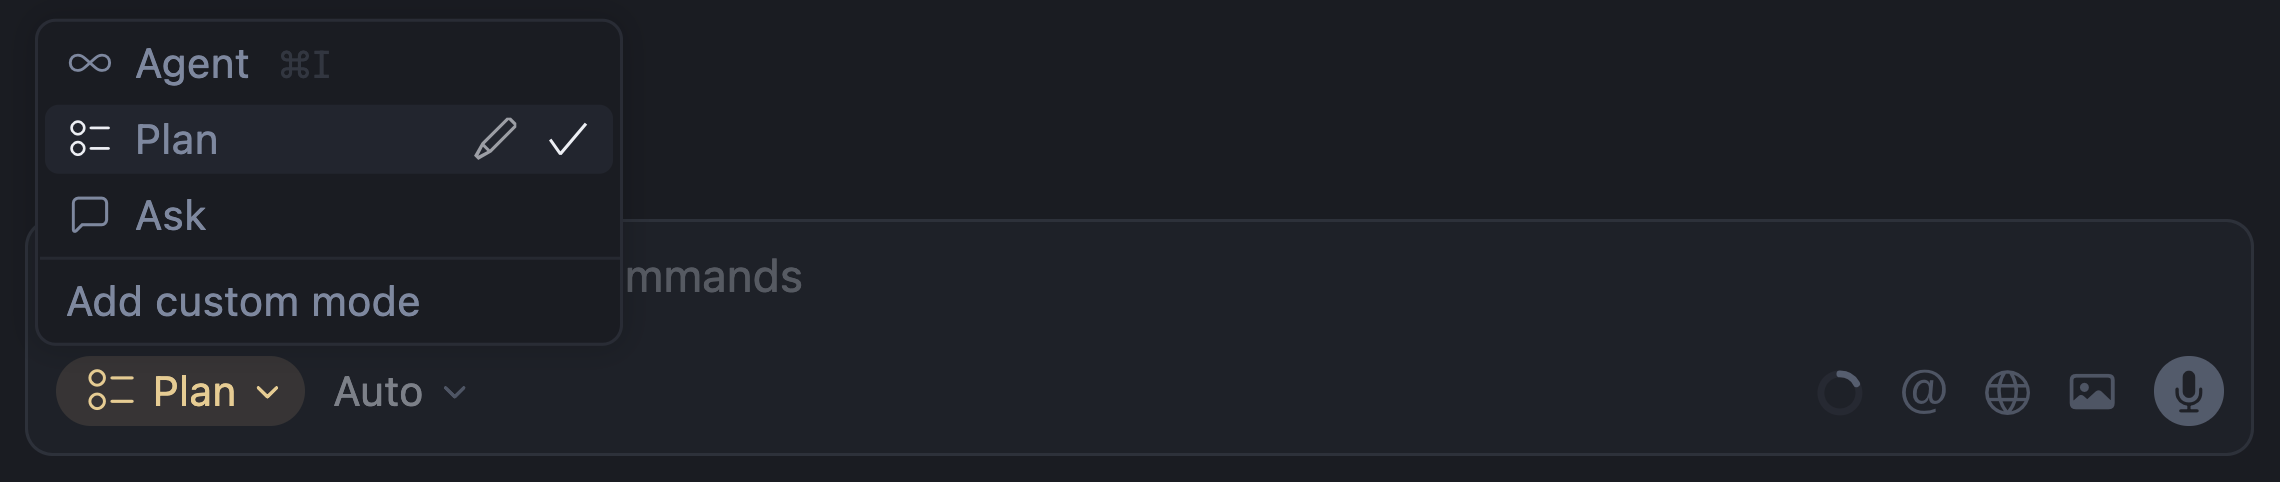
\includegraphics[width=1\textwidth]{assets/cursor/cursor-plan-mode.png}
\end{center}

\subsubsection*{Familiarization:}

Plan Mode is integrated directly into Cursor. For a brief overview, see Cursor's official \href{https://www.youtube.com/watch?v=WInPBmCK3l4}{introduction video}.

\vspace{1.2cm}
\hrule height 0.3pt
\vspace{0.7cm}

\begin{mainbox}{Important Familiarization Note}
Before starting your timed session, it is \textbf{crucial} to familiarize yourself with the features and workflows of your assigned tool by watching the provided tutorials and reviewing the relevant documentation. You are encouraged to practice using the tool on small, unrelated tasks to build confidence. However, \textbf{please avoid using the actual task or codebase during practice to minimize learning effects.}\newline\newline
\textbf{This preparation will help you use the tool effectively during the task.} In the post-session survey, you will be asked about your experience and familiarity with the tool.
\end{mainbox}

\newpage

\section{Session Workflow (Step-by-Step)}

This section explains the session workflow in which you are to attempt to complete your task. Please follow these steps in order.

\subsection{Ensure Environment is Set Up}

Following \ref{sec:your-environment}, ensure you have installed Cursor and that you have correctly set up your environment with all dependencies installed and the required repositories at the correct commit hashes. You may include the \inlinecode{PRD.md} and the \inlinecode{Prompt.md} files alongside this guide in your workspace for your convenience.\newline\newline
Opening Cursor in your designated workspace directory would look like this:
\begin{center}
    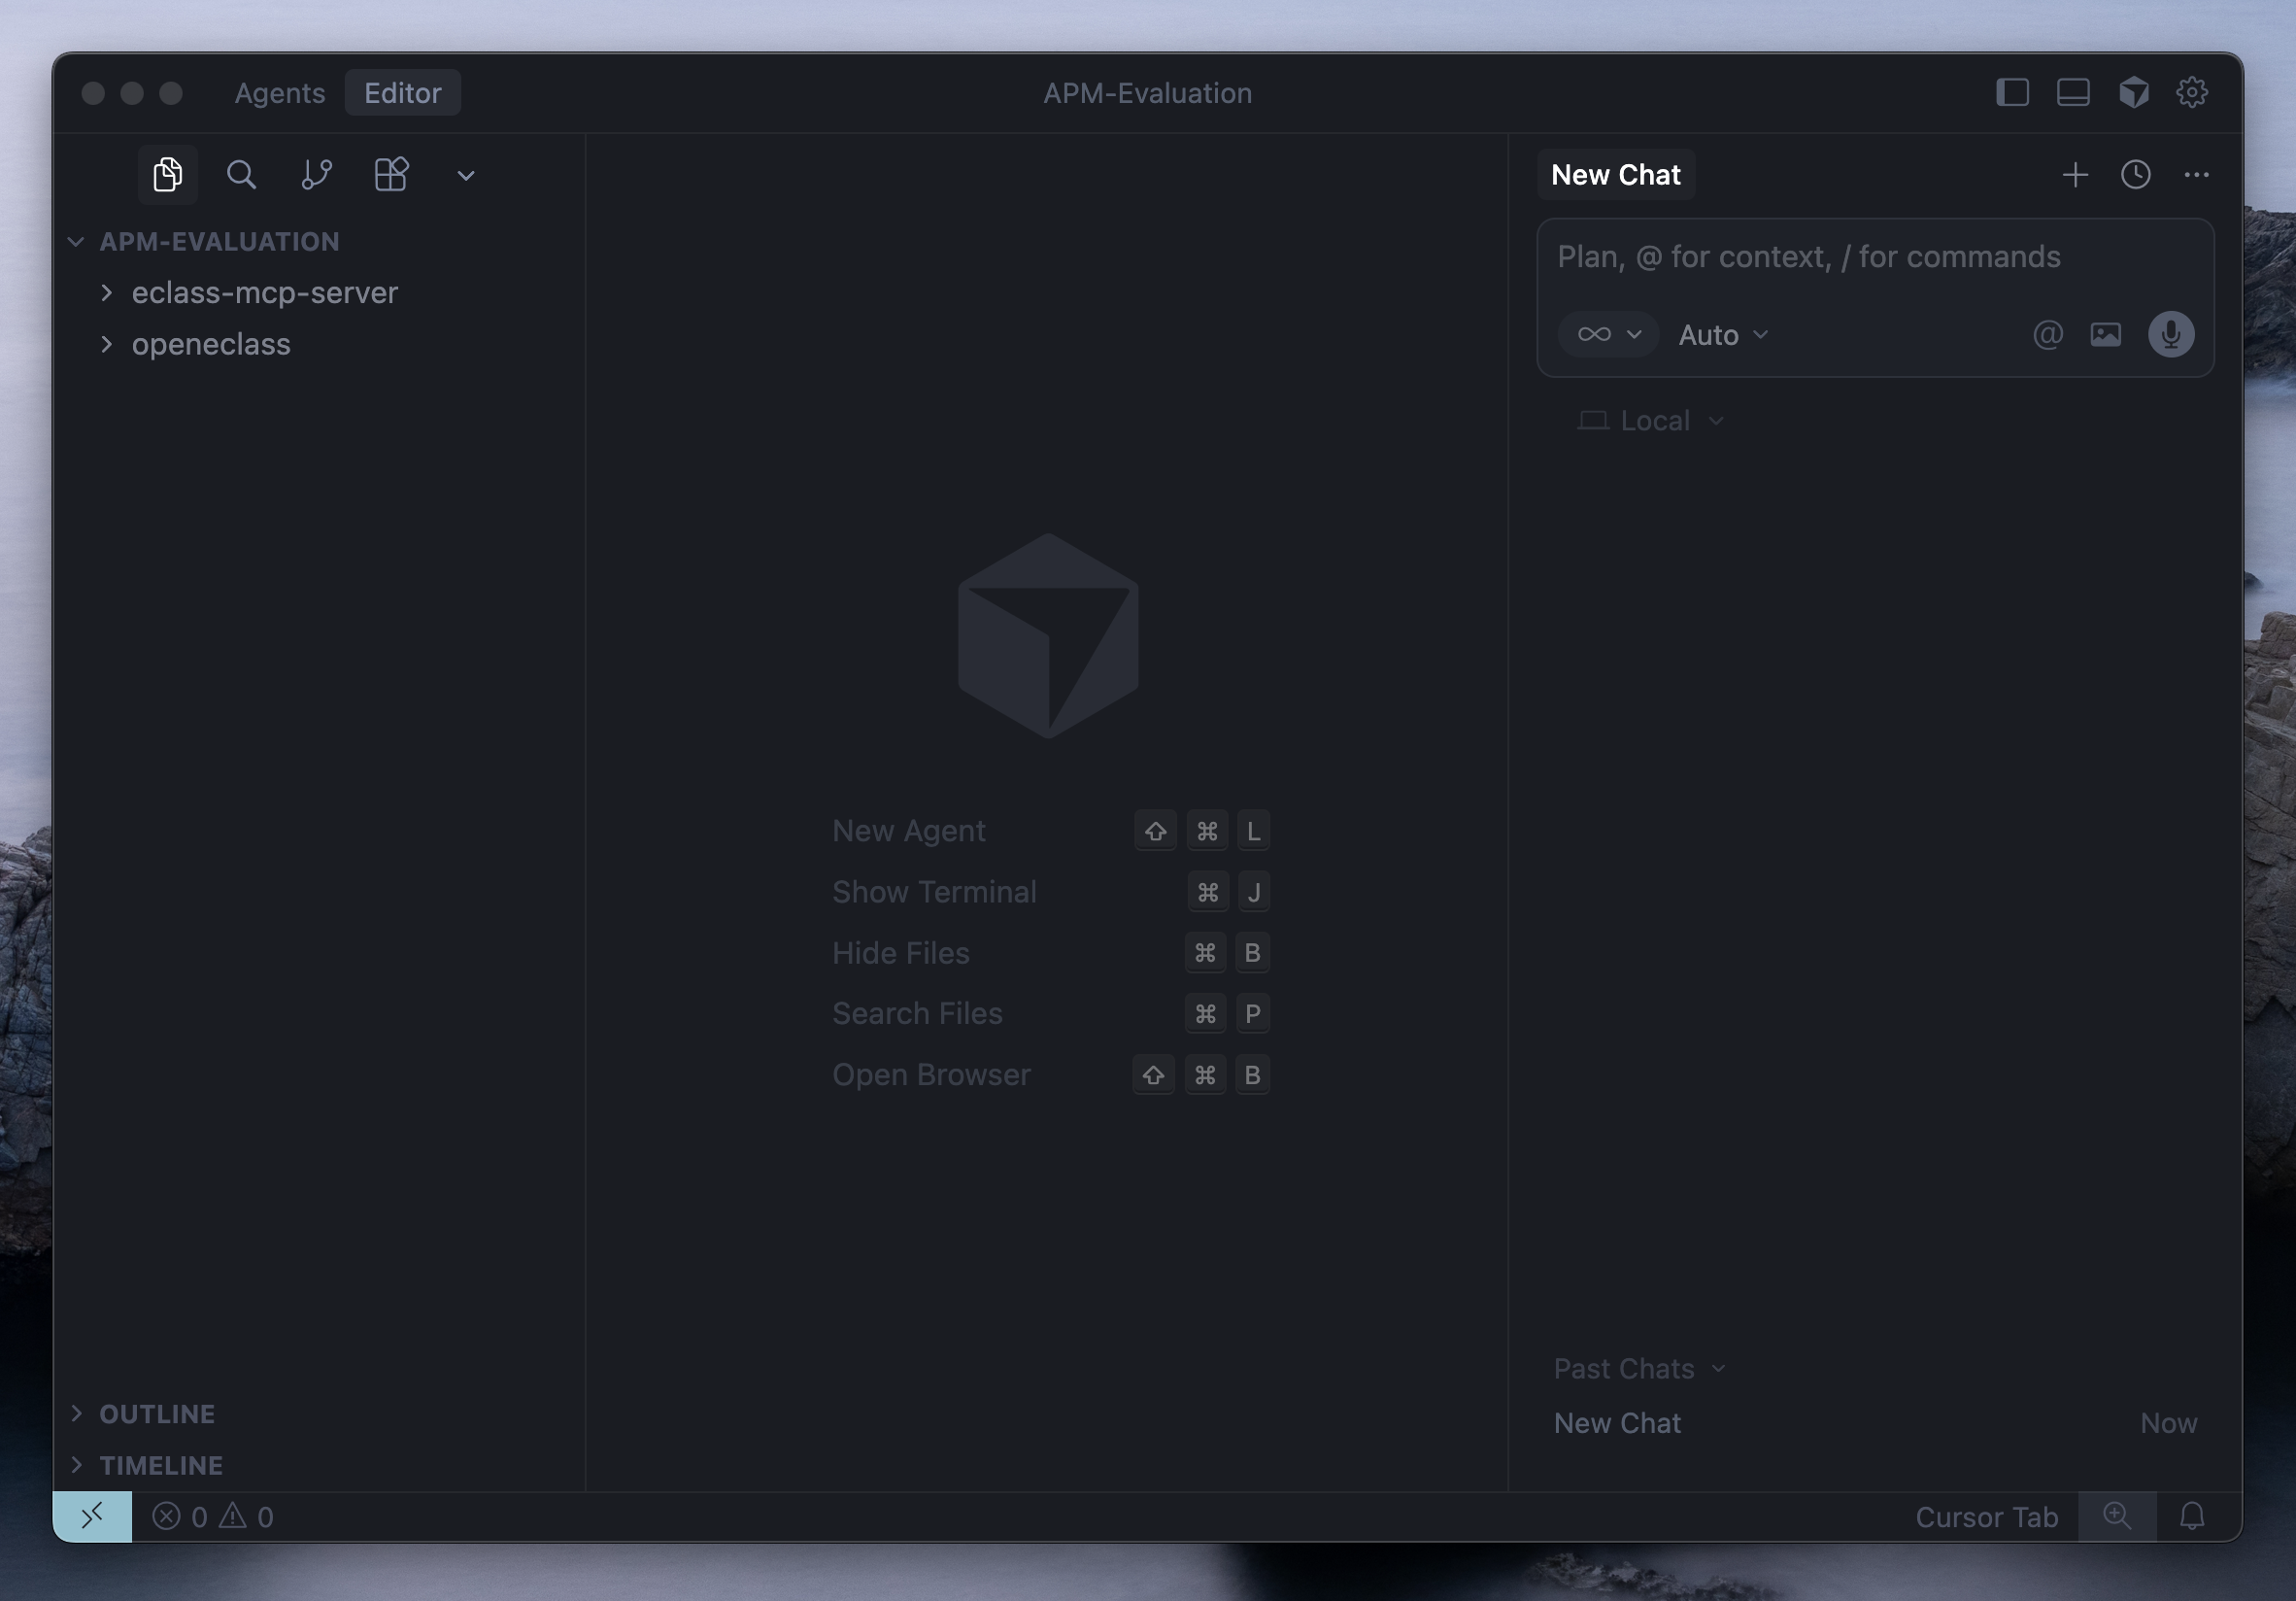
\includegraphics[width=1\textwidth]{assets/cursor/cursor-setup.png}
\end{center}

\noindent Verify that all the base dependencies are installed by running:
\begin{codebox}
/PATH/TO/PYTHON3 --version && uv --version && npm --version 

cd eclass-mcp-server && /PATH/TO/PYTHON3 -c "import mcp, requests, bs4, dotenv"

gcc --version && make --version && valgrind --version 

pkg-config --exists libcurl && pkg-config --exists libxml-2.0
\end{codebox}

\subsection{Session 1: First Tool}


\subsubsection*{Initialize Git and Create Branch:}
    
    Ensure you're starting from a clean state and create an isolated branch (replace \verb|{tool}| with your assigned tool identifier, e.g., \verb|apm|, \verb|spec-kit|, or \verb|cursor-plan|):
    \begin{codebox}
cd eclass-mcp-server                # go to implementation codebase root
git checkout main                   # switch to main branch
git checkout -b s1_{tool}           # create new branch for Session 1
    \end{codebox}

\subsubsection*{Before you start working:}
    
    \begin{itemize}
        \item Launch your first assigned AI tool following its setup instructions in \hyperref[sec:ai-tools]{Section~\ref*{sec:ai-tools}}.
        \item \textbf{Thoroughly read the} \inlinecode{PRD.md} provided alongside this guide.
        \item Use the \textbf{Default Prompt} provided alongside this guide to initiate your conversation with your AI tool.
        \item \textbf{Note the start time}; it will be used to track your session duration.
        \item Use \textbf{only} your assigned tool for AI assistance during this session.
        \item Start the timer and get to work!
        \begin{mainbox}{Important Cursor Model Selection Note}
            For study validity, all participants \textbf{must} use \textbf{Cursor's Composer 1} model for the \textbf{entire duration} of both sessions.
        \end{mainbox}
    \end{itemize}

\subsubsection*{Work Until Completion or Time Limit:}
    
    \begin{itemize}
        \item Iterate on the task for \textbf{up to 3 hours}.
        \item \textbf{Stop at the 3-hour mark}, even if you haven't completed the task.
        \item Alternatively, stop when you have fully completed the task \textbf{(if before 3 hours)}.
    \end{itemize}

\subsubsection*{Create Code Patch:}
\label{sec:creating-patch}

    After the 3 hour mark or upon completion, generate your solution patch for this session:
    \begin{codebox}
git add . && git commit -m "Session 1 solution"     
git diff main s1_{tool} > {PID}_S1_cursor_{tool}_solution.patch
    \end{codebox}

\newpage

    \begin{mainbox}{Git Note}
Feel free to use Git for version control during your session. However, ensure that you \textbf{do not modify the main branch directly}. All code changes related to your task should be committed to your isolated session branch (\texttt{s1/2\_\{tool\}}) before concluding the session.\newline

\noindent After creating the patch file, \textbf{immediately save/move it to a safe location outside your repository}. Do not delete your branch until you have saved the patch file and exported all logs; these files will be lost if you delete the branch first.
    \end{mainbox}

\subsubsection*{Export AI Interaction Logs:}

Follow the specific instructions in \hyperref[sec:exporting-logs]{Section~\ref*{sec:exporting-logs}} to export chat conversations and retrieve request statistics. Organize these in a \verb|{PID}_S1_cursor_{tool}_logs/| folder (replace placeholders with your actual values).

\subsubsection*{Clean Up and Ensure Isolation:}
    
    Return to main branch and remove the solution branch:
    \begin{codebox}
git checkout main
git branch -D s1_{tool}
    \end{codebox}
        \begin{mainbox}{Important Branch Isolation Note}
At this step, you will remove all changes made during Session 1 from your local repository. Ensure that you have successfully created the patch file, exported all logs and stored both in a safe location before proceeding, as these changes will no longer be recoverable.
        \end{mainbox}

\subsubsection*{Complete Session 1 Survey:}
\label{sec:session-1-survey}

Fill out the brief \href{https://forms.gle/dPJY5vYg6XwU4T5b8}{Session 1 post-session survey}.

\subsubsection*{Session 1 Checklist:}
\label{sec:session-1-checklist}
Before moving to Session 2, ensure you have completed the following:
\begin{itemize}
    \item Created the patch file \verb|{PID}_S1_cursor_{tool}_solution.patch| and deleted the session branch \verb|s1_{tool}|.
    \item Exported and stored all AI interaction logs:
    \begin{itemize}
        \item Exported all chat conversations as \verb|.md| chat files organized in \verb|{PID}_S1_cursor_{tool}_logs/chats/| subfolder
        \item Exported and filtered your token usage as \verb|{PID}_S1_cursor_{tool}_requests.csv| in \verb|{PID}_S1_cursor_{tool}_logs/stats/| subfolder
    \end{itemize}
    \item Completed the \href{https://forms.gle/dPJY5vYg6XwU4T5b8}{Session 1 post-session survey}.
\end{itemize}

\newpage

\subsection{Session 2: Second Tool}
\label{sec:session-2-tool-b}

Follow the same workflow as Session 1, but with the following adjustments:

\begin{itemize}
    \item Create a branch named \texttt{s2\_\{tool\}} from the clean \texttt{main} branch.
    \item Use your second assigned tool with \textbf{Cursor's Composer 1} model, following its setup instructions in \hyperref[sec:ai-tools]{Section~\ref*{sec:ai-tools}}.
    \item After the 3 hour mark or upon task, generate your solution patch for this session:
    \begin{codebox}
git add . && git commit -m "Session 2 solution"     
git diff main s2_{tool} > {PID}_S2_cursor_{tool}_solution.patch
    \end{codebox}
    \item Export and store your AI interaction logs:
    \begin{itemize}
        \item Exported all chat conversations as \texttt{.md} chat files\newline
        organized in \texttt{\{PID\}\_S2\_cursor\_\{tool\}\_logs/chats/} subfolder
        \item Exported and filtered your token usage as \texttt{\{PID\}\_S2\_cursor\_\{tool\}\_requests.csv} in \texttt{\{PID\}\_S2\_cursor\_\{tool\}\_logs/stats/} subfolder
    \end{itemize}
    \item Complete the \href{https://forms.gle/dPJY5vYg6XwU4T5b8}{Session 2 post-session survey}.
    
    \begin{mainbox}{Important Session 2 Note}
        You may start Session 2 immediately after Session 1 or take a break. Ensure you are ready to approach Session 2 from scratch, maintaining a fresh perspective and minimizing any influence from Session 1. Before starting, please \textbf{make absolutely sure you have all the artifacts from \hyperref[sec:session-1-checklist]{session 1 checklist}} safely stored.\newline\newline
        To accurately track your interaction statistics for Session 2, please \textbf{make absolutely sure you note the start time at the beginning of Session 2}. This timestamp will help isolate the request data specific to this session.
    \end{mainbox}
\end{itemize}

\subsubsection*{Session 2 Checklist:}
\label{sec:session-2-checklist}
Before concluding your work, ensure you have completed the following:
\begin{itemize}
    \item Created the patch file \verb|{PID}_S2_cursor_{tool}_solution.patch| and deleted the session branch \verb|s2_{tool}|.
    \item Exported and stored all AI interaction logs:
    \begin{itemize}
        \item Exported all chat conversations as \verb|.md| chat files organized in \verb|{PID}_S2_cursor_{tool}_logs/chats/| subfolder
        \item Exported and filtered your token usage as \verb|{PID}_S2_cursor_{tool}_requests.csv| in \verb|{PID}_S2_cursor_{tool}_logs/stats/| subfolder
    \end{itemize}
    \item Completed the \href{https://forms.gle/dPJY5vYg6XwU4T5b8}{Session 2 post-session survey}.
\end{itemize}

\newpage

\section{Exporting AI Interaction Logs from Cursor}
\label{sec:exporting-logs}

To export your AI interaction logs (chat conversations and AI request statistics) from Cursor, follow these steps for both sessions:

\subsection{Export Chat Conversations}
When using your assigned tools, you may open multiple chat conversations in Cursor (e.g., at least three with APM: Setup, Manager, and Implementation Agents; one or two with Spec-kit or Plan Mode). \textbf{Retain all chat conversations for our analysis. Do not delete any during your sessions.} To export chats, follow these steps:
\begin{itemize}
    \item For each chat conversation opened during your session, \textbf{navigate to that specific chat} so it is your \textbf{active, visible chat}.
    \item In the top-right corner of the chat window panel, click on the \textbf{three-dot options menu}.
    \item From the dropdown menu, select the \textbf{"Export Chat"} option.
    \begin{center}
        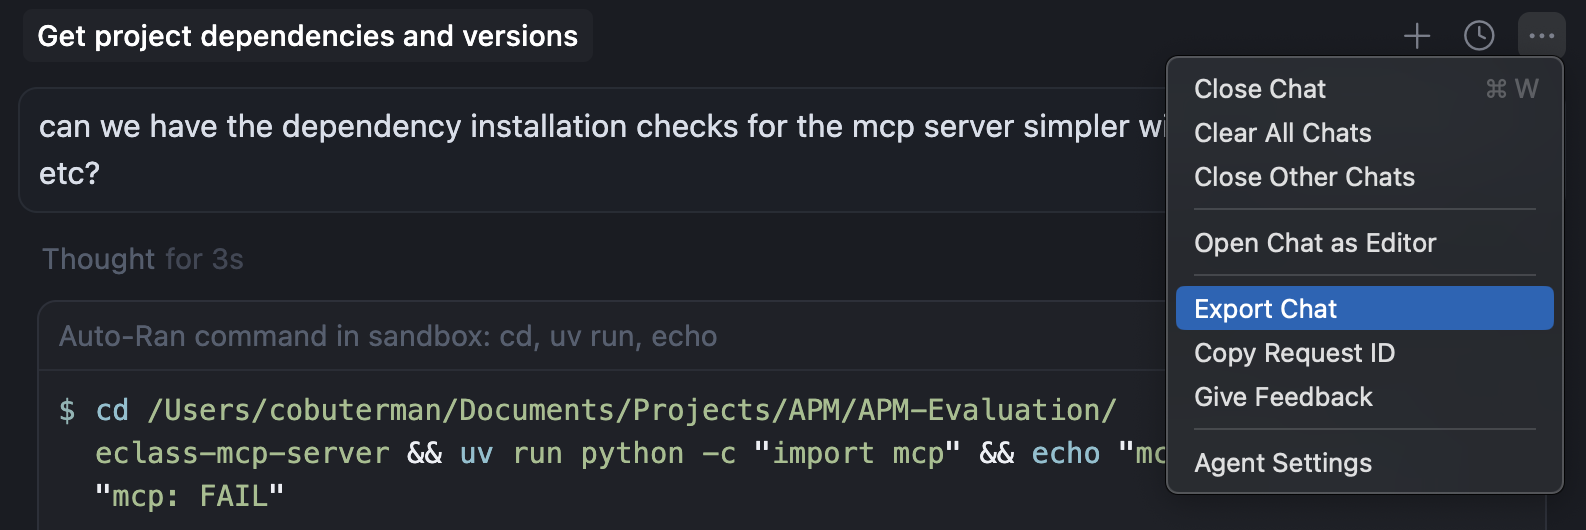
\includegraphics[width=1\textwidth]{assets/cursor/cursor-export-chat.png}
    \end{center}
    \item Save the exported \texttt{.md} file using the \textbf{strict naming format}:\newline
    \inlinecode{\{PID\}\_\{S1\textbar{}S2\}\_\{platform\}\_\{tool\}\_chat\_\{NN\}.md} where:
    \begin{itemize}
        \item \verb|{PID}| is your participant ID (e.g., \verb|P001|), 
        \item \verb|{S1/2}| is the session number,
        \item \verb|{platform}| is \verb|cursor|,
        \item \verb|{tool}| is your assigned tool identifier (e.g., \verb|apm|, \verb|spec-kit|, \verb|cursor-plan|),
        \item \verb|{NN}| is the chat number starting from \verb|01| (e.g., \verb|P001_S1_cursor_apm_chat_01.md|, \verb|P001_S1_cursor_apm_chat_02.md|).
    \end{itemize}
\end{itemize}
\noindent Repeat this process for all conversations used during the session.
\begin{mainbox}{Important Chat Export Note}
    To take extra precautions, consider exporting conversations \textbf{immediately after completion} to avoid accidental deletions or technical issues. For example, in APM the Setup Agent conversation can be exported right after the Setup Phase is complete.
\end{mainbox}

\newpage

\subsection{Retrieve AI Request Statistics}

To retrieve your AI request statistics from Cursor, follow these steps:

\begin{itemize}
    \item Login to your \href{https://cursor.com}{Cursor} account and go to the \href{https://cursor.com/dashboard}{Cursor Dashboard}.
    \item On the sidebar, click on the \textbf{"Usage"} tab to access your usage statistics. 
    \item Click on the \textbf{"Export CSV"} button located at the top-right corner of the Usage page.
    \begin{center}
        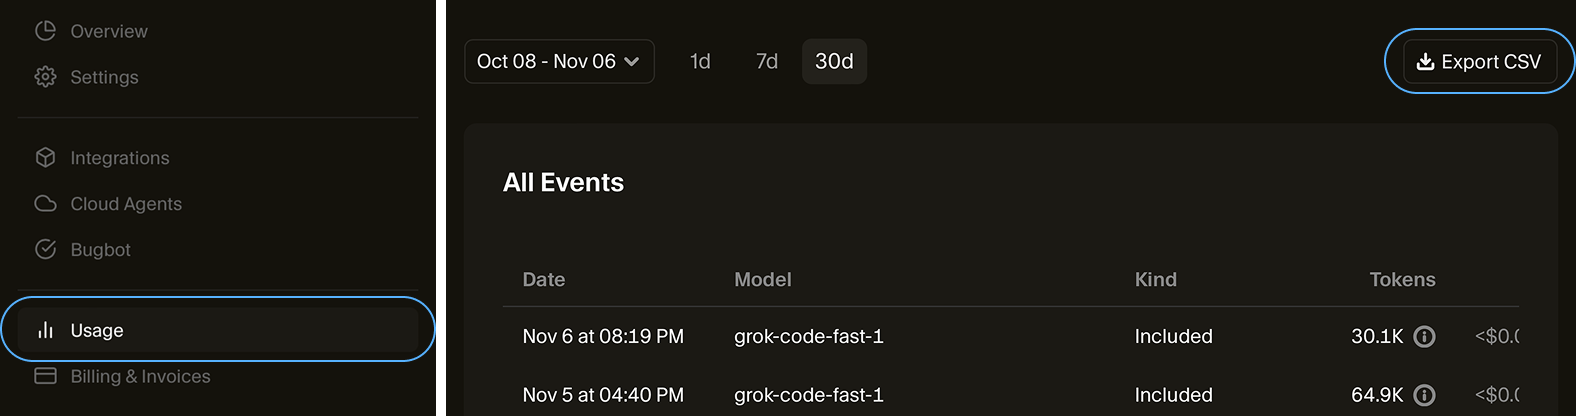
\includegraphics[width=1\textwidth]{assets/cursor/cursor-dashboard.png}
    \end{center}
\end{itemize}

\noindent This will immediately download a CSV file containing your AI request statistics to your local machine. This file contains AI requests made across all your sessions. \newline

\noindent To isolate the requests made during your specific session, use the provided python script\newline\texttt{filter\_csv\_by\_datetime.py} with the \textbf{start time} you noted at the beginning of each session and rename the output file using the \textbf{strict naming format} (e.g., \inlinecode{P001\_S1\_cursor\_apm\_requests.csv}). \newline

\noindent For example, if your session started on 2025-11-06 at 14:30 in the Europe/Athens timezone:
\begin{codebox}
python3 filter_csv_by_datetime.py usage-events.csv 2025-11-06 14:30 Europe/Athens
\end{codebox}

\begin{mainbox}{Important Timing Note}
This will create a filtered CSV file containing only requests from that point onward (e.g.,\newline \texttt{usage-events\_filtered\_2025-11-06\_14:30\_Europe\_Athens.csv}).\newline\newline
Run the filtering script \textbf{immediately after completing your session} to ensure the CSV includes all requests from the session start up to your last AI request. If you wait too long before filtering, additional requests from other activities may be included.
\end{mainbox}

\newpage

\subsection{Organize Logs for Submission}

Save the exported chat conversations and filtered request statistics in a dedicated logs folder. Create the following folder structure using your participant ID, session number, platform, and tool identifier:

\begin{codebox}
{PID}_S1_cursor_{tool}_logs/
    chats/
        {PID}_S1_cursor_{tool}_chat_01.md
        {PID}_S1_cursor_{tool}_chat_02.md
        ...
    stats/
        {PID}_S1_cursor_{tool}_requests.csv
\end{codebox}

\section{Final Submission}

After completing a session, organize your patch file and logs folder for submission.

\subsection{Create Submission Zip Files}

Once you have your patch file and organized logs folder for each session, create the final submission zip files using the correct naming format:
\begin{codebox}
# For Session 1
zip -r {PID}_S1_cursor_{tool}_submission.zip {PID}_S1_cursor_{tool}_solution.patch {PID}_S1_cursor_{tool}_logs/

# For Session 2
zip -r {PID}_S2_cursor_{tool}_submission.zip {PID}_S2_cursor_{tool}_solution.patch {PID}_S2_cursor_{tool}_logs/
\end{codebox}

\begin{mainbox}{Important Submission Note}
Ensure both the patch file and logs folder are at the root level of your zip file (not in subdirectories). The zip file should contain exactly two items: the \texttt{.patch} file and the \texttt{\{PID\}\_\{S1\textbar{}S2\}\_cursor\_\{tool\}\_logs/} folder. Use the strict naming format \texttt{\{PID\}\_\{S1\textbar{}S2\}\_\{platform\}\_\{tool\}\_submission.zip} as shown above. Only \texttt{\{PID\}} and \texttt{S} are uppercase; all other components must be lowercase.
\end{mainbox}

\noindent After completing both sessions, submit all your data to our \href{https://forms.gle/gzYNsSZwMbUDJRji6}{anonymous collection form}.

\newpage

\subsection*{Submission Checklist}

Please be sure to upload the following single \inlinecode{.zip} files (one for each session):

\begin{itemize}
    \item \verb|{PID}_S1_cursor_{tool}_submission.zip| \newline Contains: \verb|{PID}_S1_cursor_{tool}_solution.patch + {PID}_S1_cursor_{tool}_logs/|
    \item \verb|{PID}_S2_cursor_{tool}_submission.zip| \newline Contains: \verb|{PID}_S2_cursor_{tool}_solution.patch + {PID}_S2_cursor_{tool}_logs/|
\end{itemize}

\section{Contact \& Help}

This study is conducted for a Bachelor's thesis by Kostantinos Chaidemenos - \href{https://github.com/sdi2200262}{CobuterMan}.\newline\newline
If you encounter any technical issues or have questions about the study procedure, contact: 
\begin{codebox}
sdi2200262@di.uoa.gr        # Email
cobuter_man                 # Discord
\end{codebox}

\vspace{1cm}
\hrule height 0.3pt
\vspace{0.7cm}

\begin{center}
    \subsubsection*{\centering Thank you again for your time and contribution to this research.}
    
\includegraphics[width=0.3\textwidth]{assets/common/cobuter-man.png}
\end{center}

% ============================================================================

\end{document}
